\section{Control-Flow Analysis}
\begin{itemize}
  \item If functions are introduced as values i.e. higher-order functions or object with methods, then the control flow and data flow suddenly become intertwined
  \begin{itemize}
  	\item It is no longer trivial to see which code is being called
  	\item The task of \textbf{control flow analysis} is to conservatively approximate the interprocedural control flow (call graph) for such programs
  \end{itemize}
\end{itemize}
\subsection{Closure analysis for $\lambda$-calculus}
\begin{itemize}
  \item Control flow analysis in its purest form is best illustrated by $\lambda$ calculus
  \begin{align*}
    E &\to \lambda X.E \\
    & \mid \quad X \\
    & \mid \quad E E
  \end{align*} 
  \item To construct a CFG for a term in this calculus every expression $E$ needs to be approximated to the set of \textbf{closures} to which it may evaluated
  \begin{itemize}
  	\item It can be modeled by a symbol of the form $\lambda X$ that identifies a concrete $\lambda$ abstraction
  	\item The problem is called \textbf{closure analysis}
  	\item The lattice used is the powerset of closures occurring in the given term and ordered by subset inclusion
  	\item For every AST node $v$ a constraint variable $\co{v}$ is used to denote the set of resulting closures
  \end{itemize}
  \item For an abstraction $\lambda.E$ we have the following constraint
  \begin{equation*}
    \lambda X \in \co{\lambda X.E}
  \end{equation*}
  \item For an application $E_1E_2$ we have the following conditional constraint
  \begin{equation*}
    \lambda X \in \co{E_1} \Rightarrow (\co{E_2} \subseteq \co{X} \land \co{E} \subseteq \co{E_1E_2}) 
  \end{equation*}
\end{itemize}

\subsection{The Cubic Algorithm}
\begin{figure}[H]
	\centering
	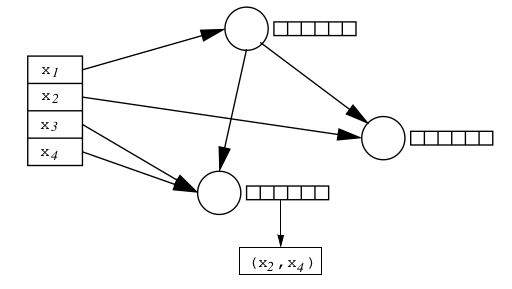
\includegraphics[width=220pt]{img/control_flow/cubic_graph}
\end{figure}

\begin{itemize}
  \item Given a finite set of \textbf{tokens} $\{t_1,\dots,t_k\}$ and a finite set of \textbf{variables} $x_1,\dots,x_n$ whose values are set of tokens the task is to read a collection of constraints on the form $t \in x$ or $t \in x \Rightarrow y \subseteq x$ and produce a minimal solution
  \begin{itemize}
  	\item Each variable is mapped to a node in a DAG
  	\item Each node has an associated bit vector $\in \{0,1\}^k$
    \begin{itemize}
  		\item Initially all 0's
    \end{itemize}
  	\item Each bit has an associated list of pairs of variables, which is used to model conditional constraints
  	\item The edges in the DAG reflect inclusion constraints.
  	\item Constraints are added one at a time
  	\item The bit vectors will at all times directly represent the minimal solution of the constraints seen so far
  	\item A constraint of the form $t \in x$ is handled by
    \begin{enumerate}
		  \item Looking up the node associated with $x$ and setting the corresponding bit to $1$
		  \item If its list of pairs was not empty then an edge between the nodes corresponding to $y$ and $z$ is added for every pair $(y,z)$
    \end{enumerate}
  	\item A constraint of the form $t \in x \Rightarrow y \subseteq z$ is handled by first testing if the bit corresponding to $t$ in the node corresponding to $x$ has value $1$
    \begin{itemize}
  		\item If so then an edge between the nodes corresponding to $y$ and $z$ are added
  		\item Otherwise the pair $(y, z)$ is added to the list for that bit
    \end{itemize}
  	\item If an added edge creates a cycle the corresponding nodes can be merged into one node
    \item To reestablish all inclusion constraints the values of each newly set bit must propagate through all edges in the graph
  \end{itemize}
  \item The running time of the algorithm is $O(n^3)$
\end{itemize}

\subsection{TIP with first class functions}
\begin{itemize}
  \item If TIP allows functions as values then for a computed function call
  \begin{equation*}
    E \to E(E_1, \dots, E_n)
  \end{equation*}
  one can no longer see directly from the syntax which functions may be called
  \item The lattice is the powerset of the set of tokens containing $X$ for every function name $X$ ordered by subset inclusion
  \item For a function named $f$ the following constraint is used
  \begin{equation*}
    f \in \co{f}
  \end{equation*}
  For an assignment $X = E$ the following constraint is used
  \begin{equation*}
    \co{E} \subseteq \co{X}
  \end{equation*}
  \item For computed function calls $E(E_1, \dots, E_n)$ then for every definition of a function $f$ with arguments $a_f^1, \dots, a_f^n$ and return expression $E_f^\prime$ the following conditional constraint is added
  \begin{equation*}
    f \in \co{E} \Rightarrow (\co{E_1} \subseteq \co{a_f^1} \land \cdots \land \co{E_1} \subseteq \co{a_f^1} \land \co{E_f^\prime} \subseteq \co{E(E_1, \dots, E_n)})
  \end{equation*}
\end{itemize}

\newpage
%%% Local Variables:
%%% mode: latex
%%% TeX-master: "pav-noter"
%%% End:
